% 中文平行版中期报告：结构、数字、图表与 interim_report.tex 完全一致。
% 编译（LM2，两遍）：export PATH=/data6/jinxinhao/texlive/2026/bin/x86_64-linux:$PATH
%   xelatex interim_report_zh.tex && xelatex interim_report_zh.tex
\documentclass[11pt]{article}
\usepackage[margin=1in]{geometry}
\usepackage{amsmath,amssymb}
\usepackage{booktabs}
\usepackage{graphicx}
\usepackage{xcolor}
\usepackage{xeCJK}
\setCJKmainfont{FandolSong-Regular}[
  Extension = .otf, BoldFont = FandolSong-Bold,
  AutoFakeBold = 2.2, AutoFakeSlant = 0.2]
\setCJKsansfont{FandolHei-Regular}[Extension = .otf, AutoFakeBold = 2.2]
\renewcommand{\figurename}{图}
\renewcommand{\tablename}{表}
\renewcommand{\abstractname}{摘要}
\renewcommand{\refname}{参考文献}
\usepackage[hidelinks]{hyperref}
\emergencystretch=3em

\title{\bfseries PanNuke 上的稀有细胞核是一个检测问题：\\
诊断、两个失败的数据侧修复，与反事实压力测试\\[6pt]
\large 中期报告（课程项目 bdd26）}
\author{金鑫豪（Xinhao Jin）}
\date{2026 年 9 月 28 日}

\begin{document}
\maketitle

\begin{abstract}
在 PanNuke 上，更换 backbone 只能带来 1--2 个 mPQ 点的收益，而\textbf{Dead}（凋亡）类
的 PQ 在所有已发表模型中停滞在 0.13--0.18。本中期报告回答两个问题：为什么，以及病理
视觉--语言模型与可控生成模型这两类“新范式”能否改善稀有类缺陷，或改进鲁棒性评测。我们首先
在官方 3-fold 协议下复现两个基线（HoVer-Net 0.456 mPQ、CellViT-UNI 0.500），并加入第三
个评估器 HoVer-NeXt-T（0.458）——其初始移植得分 0.358 被证明是解码伪影而非模型差距。
其次，我们证明 Dead 缺陷集中于\textbf{检测}而非分类：38.5\% 的 Dead 真值核没有任何重
叠预测；在这些漏检核内部，前景头沉默（平均核概率 0.16），而类型头却给出
P(Dead)$\approx$0.26。第三，在预注册的多种子协议下，四类干预全部无效或有害：病理 VLM
（CONCH）后处理重分类、免训练漏检找回、类别/尺寸加权的前景损失，以及数据侧的失败驱动
copy-paste（Dead PQ $-0.031$）与标签自洽的上下文内扩散合成（mPQ 持平）。第四，我们构建
了三架构 $\times$ 三数据集的零样本跨域基准（CoNIC、MoNuSAC、PUMA）与
\emph{PanNuke-CF}——固定 PanNuke 标签、对组织上下文与染色做干预后重渲染的反事实测试
集。反事实压力测试\textbf{反转}了真实跨域排序（6 个评估点 Spearman $-0.89$；架构均值
$-1.00$）：轴分解显示架构间的真实迁移差异几乎全部位于检测轴，而标签固定的渲染在构造
上无法对检测施压；在它能施压的分型轴上，反事实排序与真实迁移一致。结论：反事实渲染是
有效的\emph{分型}压力测试而非迁移代理；Dead 检测缺陷是架构性的——它对我们测试的所有
损失级与数据级干预都免疫，并且跨域依然存在（三架构在 PUMA 上 Dead PQ $\le 0.006$）。
\end{abstract}

\section{引言}
\label{sec:intro}

细胞核实例分割与分类是计算病理学的标准任务，PanNuke~\cite{gamper2019pannuke} 是其标准
基准：19 种组织、205,000 个标注核，以组织平均 mPQ（mean panoptic quality）评测。其排行榜
呈现出失衡的格局：五年的架构进步只换来约 1--2 个 mPQ 点
（HoVer-Net~\cite{graham2019hovernet} 0.463 $\rightarrow$
CellViT-SAM-H~\cite{horta2024cellvit} 0.498 $\rightarrow$ 当前最佳约 0.51），而
\emph{Dead}（凋亡小体）类始终停在 PQ 0.13--0.18，粘连核的 merge/split 错误也持续存在。
两类新范式有望带来比 backbone 工程更大的收益：病理视觉--语言
模型~\cite{lu2024conch}作为类型分类的先验，与可控生成模型~\cite{le2025pixcell}作为
“组织模拟器”（定向合成训练数据，或在干预下重渲染评测图像）。

本项目按三个预注册支柱组织，附明确的通过/失败规则——其逻辑是：负结果只有在验收标准
事先固定时才有价值。\textbf{A}：语言锚定的类型头（用 CONCH 文本空间攻击稀有类
\emph{分类}）；\textbf{B}：失败驱动的合成（用生成数据攻击 Dead/小核\emph{检测}）；
\textbf{C}：评测（用真实跨域迁移加反事实测试集攻击鲁棒性度量）。三个支柱现均已收官；
本报告记录其发现。贡献如下：

\begin{enumerate}
\item \textbf{单一严格协议下的复现}（\S\ref{sec:setup}）：HoVer-Net、CellViT-UNI、
HoVer-NeXt-T 以完全相同的方式在官方 3-fold 划分上训练与评测：last checkpoint、解码仅在验
证折上调节。顺带量化了一个已发布评测配方（16 个随机颜色 TTA 视图 + 在\emph{测试折}上
调阈值）能抬高多少分数（\S\ref{sec:baselines}）。
\item \textbf{Dead 缺陷的分解}（\S\ref{sec:diagnosis}）：它是一个集中在小核与孤立核上
的\emph{检测}失败——前景头看不见，类型头却部分“看见”——这正是所有类型侧干预都失败的原因。
\item \textbf{预注册的负结果}（\S\ref{sec:pillarA}、\S\ref{sec:pillarB}）：CONCH 重分
类、免训练找回、损失重加权（3 种子）、失败驱动 copy-paste、上下文内扩散合成全部无效或
有害；并给出了种子噪声标定，说明多大的效应量才可信。
\item \textbf{$3{\times}3$ 架构 $\times$ 数据集零样本跨域基准}（\S\ref{sec:external}），
其中 PUMA 是我们所能找到的唯一较大规模的外部凋亡 Dead 标签来源；CoNIC 与 MoNuSAC 的
转换与核验管线一并给出。
\item \textbf{PanNuke-CF}：标签固定的反事实渲染基准（\S\ref{sec:cf}），其有效性分析在
机理层面给出判定：外观反事实无法探测检测（这是构造上的限制），因此在 mPQ 层面\emph{反转}真实迁
移排序，但作为分型压力测试仍然有效。
\end{enumerate}

所有结果来自同一代码库与同一评测器；该评测器已对官方 PanNuke-metrics 做到逐位一致
（官方发布的 \texttt{class\_stats.csv} 存在列交换 bug，已在仓库中记录）。

\section{相关工作}
\label{sec:related}

\paragraph{PanNuke 模型。}HoVer-Net~\cite{graham2019hovernet} 提出的水平--垂直
watershed 解码至今仍被多数后续工作（以变体形式）沿用。CPP-Net~\cite{cppnet}、
HoVer-NeXt~\cite{hovenext}、CellViT~\cite{horta2024cellvit} 及其后续
（LKCell、CellVTA、CellViT++~\cite{horta2025cellvitpp}）、
PromptNucSeg~\cite{promptnucseg} 填满了 0.46--0.51 的 mPQ 区间。其中只有部分工作发布了
按折权重；若官方权重在全量数据上训练（如 HoVer-Net 官方权重），则只能作管线 sanity
check，绝不能作为测试结果——本报告全程执行这一区分。

\paragraph{病理基础模型与 VLM。}冻结病理基础模型在稠密任务上并不自动胜过 ImageNet
CNN~\cite{mindthegap}；病理 VLM CONCH~\cite{lu2024conch} 在稠密预测上与纯视觉模型持平，
但额外提供对齐的文本空间。纯提示接口在细胞核任务上表现极差（SAM3 式提示在 PanNuke 类任务
上 mIoU $<10\%$）；最接近的已有工作（PromptNu、MONCH）要么没有官方 PanNuke 配置，要么
只做语义分割。我们未找到“病理 VLM 文本空间 + 实例分割 + 官方 PanNuke mPQ”的先前工作。

\paragraph{生成式增强与压力测试。}已有报道合成数据对\emph{稀有类}有帮助
（DiffMix、HistoSmith、NucleiMix~\cite{nucleimix}），但据我们所知没有工作在官方 3-fold
PanNuke 协议下以 mPQ 报告；已有研究使用非标准划分与 Dice/AJI/F1。影像模型的反事实压力
测试已在放射学中得到演示~\cite{cfstress}；我们不知道实例分割的对应工作。PixCell~\cite{le2025pixcell}
（连同其 Cell-ControlNet）是当前最强的开源可控细胞核生成器，是我们合成实验与反事实渲
染器的共同底座。

\section{实验设置}
\label{sec:setup}

\paragraph{数据与协议。}PanNuke 第 1--3 折，官方划分（train/val/test $=1/2/3$、
$2/1/3$、$3/2/1$）；所有数字为 \emph{last-checkpoint} 模型的 3-split 均值，不做基于测试
集的早停。外部数据集（\S\ref{sec:external}）为零样本：每个数据集固定到 PanNuke 5 类的
类别映射，缺失类按官方协议从 mPQ 中排除。

\paragraph{指标。}官方组织平均 mPQ/bPQ（对 PanNuke-metrics 的逐位一致复现）、strict mPQ
（对图中不存在类的 FP 计罚而非忽略）、AJI/AJI$^+$、检测 $F_d$ 与分类 $F_c$（12\,px 质心
匹配）、以及 IoU 0.5 的错误分解（matched / merged / missed-no-overlap /
missed-poor-shape / split，按类拆分）。TTA（8 个二面体变换，HV 通道重映射）单独报告。

\paragraph{噪声标定（用于每个判定）。}同一 CellViT-UNI 配方的 3 个种子：种子 std 在
mPQ 上为 0.0021，但在 Dead PQ 上为 \textbf{0.0074}；Dead 的图像 bootstrap CI 半宽为
0.02--0.03。我们据此执行以下规则：单种子 Dead 变化低于约 0.01--0.015 视为噪声；每个干预的判定
必须是 3 种子（或多折）结论，附配对、组织分层图像 bootstrap 95\% CI；决策只在验证折上
做。

\subsection{基线}
\label{sec:baselines}

\begin{table}[t]
\centering\small
\caption{官方 3-fold 协议下的基线（3-split 均值；last checkpoint；无 TTA，TTA 在括号
内）。“已发表”= 论文自报数字（其各自配方）。}
\label{tab:baselines}
\begin{tabular}{lccc}
\toprule
模型 & mPQ & bPQ & Dead PQ \\
\midrule
HoVer-Net（本文）      & .4564 [.4666] & .6613 [.6714] & .127 [.128] \\
\quad 已发表            & .463 & .660 & .139 \\
CellViT-UNI（本文）    & .4995 [.5047] & .6654 [.6706] & .176 [.177] \\
\quad 已发表（CellViT++）& .492 & .664 & .154 \\
HoVer-NeXt-T（本文）   & .4579 & .6367 & .136 \\
\quad 已发表            & .477 & .656 & .154 \\
\bottomrule
\end{tabular}
\end{table}

表~\ref{tab:baselines}：两个经典基线都成功复现（HoVer-Net 略低于原文，与常见复现一致；
CellViT-UNI 略高于原文）。HoVer-NeXt-T 需要移植，初始得分仅 0.358 mPQ；消融表明
\emph{预测图本身没有问题}，性能损失完全出在解码环节。其发布的 0.477 配方平均 16 个随机空间
+\emph{颜色} TTA 视图，并在\emph{测试折}上调每类阈值。我们改用它自身的验证解码（平坦
fg/seed 阈值），只在每个 split 的\emph{验证}折上调参——与其它基线同一协议——得到
0.4579。二者之差（0.458 vs 0.477）反映了测试侧调参与随机颜色 TTA 一共能带来多少提升；
这个量级（0.02 mPQ）大于排行榜上多数名次差距。HoVer-NeXt-T 作为第三评估器的价值在于
\emph{不同的错误画像}：三者中 merge 率最低（0.096--0.101，HoVer-Net 约 0.14），
missed-background 更高。

\section{支柱 A：Dead 缺陷是检测缺陷}
\label{sec:pillarA}

\subsection{CONCH 语义存在于上下文尺度（可行性）}
对真值核的零样本 CONCH 分类：紧裁剪接近随机（32\,px：0.27），全上下文 patch 加半径受限
注意力池化达到平衡准确率 0.695（R\,=\,32\,px，每 patch 一次前向）；LLM 形态学描述比纯类
名高 8--11 个点。Dead 是\emph{最}可被文本识别的类（召回 0.88），却也是分割模型最差的
类——但在自然分布下其零样本精度仅约 0.10，只能作为互补信号。线性头的文本锚定初始化只在
少样本情形（每类 $\le$25 核）下有帮助；全量 PanNuke 标注下无关紧要。这把支柱 A 的重心从分类
转移到了检测。

\subsection{管线内重分类：无效}
把 CONCH（零样本或线性探针）融合进 CellViT-UNI 的类型决策，所有可调参数均在验证折上确定
（表~\ref{tab:retype}）：没有任何配置超过管线自身的 seg-vote 类型；重校准对照与最佳融
合持平。TTA 下，验证调参为两种融合都选择了 $\alpha=0$。

\begin{table}[t]
\centering\small
\caption{CellViT-UNI 上的后处理重分类，split 1（测试折 3）。}
\label{tab:retype}
\begin{tabular}{lccc}
\toprule
方法 & val mPQ & test mPQ & test Dead PQ \\
\midrule
seg vote（管线）                 & .4835 & .4951 & .142 \\
+ 类别偏置重校准                 & .4873 & .4953 & .135 \\
$\times$ CONCH 零样本（$\alpha{=}.1$） & .4835 & .4938 & .141 \\
$\times$ CONCH 线性（$\alpha{=}.3$）    & .4836 & .4920 & .141 \\
CONCH 线性单独                   & .3645 & .3821 & .145 \\
\bottomrule
\end{tabular}
\end{table}

\subsection{免训练找回：无效}
在原始 NP/HV/TP 图上扫描 96 个配置（前景混合、Dead 先验增强、blob 阈值、孤立体找回；
3 splits，验证集选择）：每个族与仅调阈值的对照差距在 $\pm0.0004$ test mPQ 之内。漏检
的 Dead 核无法从该模型的输出中找回。

\subsection{损失侧消融：无效或是交换}
split 1 上的像素加权前景 CE，配 3 种子基线：Dead 像素权 $\times$11（M1）无效；完全均衡
采样器（C1）无效；小核权 $\times$6（M2）在一个种子里看似有希望（$+0.0042$ test mPQ，
CI 不含 0），但 3 种子上 mPQ $-0.0010$ $[-0.0043,+0.0022]$，且 bPQ \emph{显著}下降
$-0.0024$ $[-0.0048,-0.0002]$，Dead 增益 $+0.0108$ $[-0.0021,+0.0238]$ 不显著——这是一
次交换而非贡献；它也清楚地表明，在该基准上低于约 0.004 的单种子 mPQ 效应就是种子运气。

\subsection{诊断：Dead 性能在哪里丢失}
\label{sec:diagnosis}

\begin{table}[t]
\centering\small
\caption{CellViT-UNI 在折 3 上的错误分解（IoU 0.5；真值核占比）。}
\label{tab:decomp}
\begin{tabular}{lcccccc}
\toprule
真值类 & matched & merged & missed & miss(形状) & split & 匹配后类型正确 \\
\midrule
Neoplastic   & .811 & .048 & .092 & .040 & .009 & .905 \\
Inflammatory & .849 & .046 & .079 & .023 & .004 & .817 \\
Connective   & .752 & .038 & .153 & .044 & .013 & .794 \\
Dead         & \textbf{.470} & .089 & \textbf{.385} & .048 & .008 & .690 \\
Epithelial   & .837 & .042 & .075 & .036 & .011 & .930 \\
\bottomrule
\end{tabular}
\end{table}

表~\ref{tab:decomp}：38.5\% 的 Dead 核\emph{没有任何重叠预测}（其它类 8--15\%），而
Dead 匹配后类型正确率为 0.69——性能损失首先出在检测。在漏检的 Dead 核内部，前景头沉默（平均
NP 概率 0.164，仅在 17\% 的核中有响应），类型分支却给出 P(Dead)\,$\approx$\,0.26（其它类漏检核约
0.01）：网络其实“看见”了这些凋亡物质，只是前景头没有给出响应。尺寸是重要因素（Dead 中位面积 107\,px，其它类
368；24\% 的 Dead $<$60\,px，其它类 6\%），但外观效应在尺寸分层后依然存在：大 Dead
（$>$200\,px）的漏检率是其它大类核的 6 倍（0.214 vs 0.035）。定性上
（图~\ref{fig:dead}），漏检 Dead 是核碎裂碎片、乏染色质的嗜酸性小体与模糊标注。结论：
要么改检测，要么改数据——由此定义支柱 B。

\begin{figure}[t]
\centering
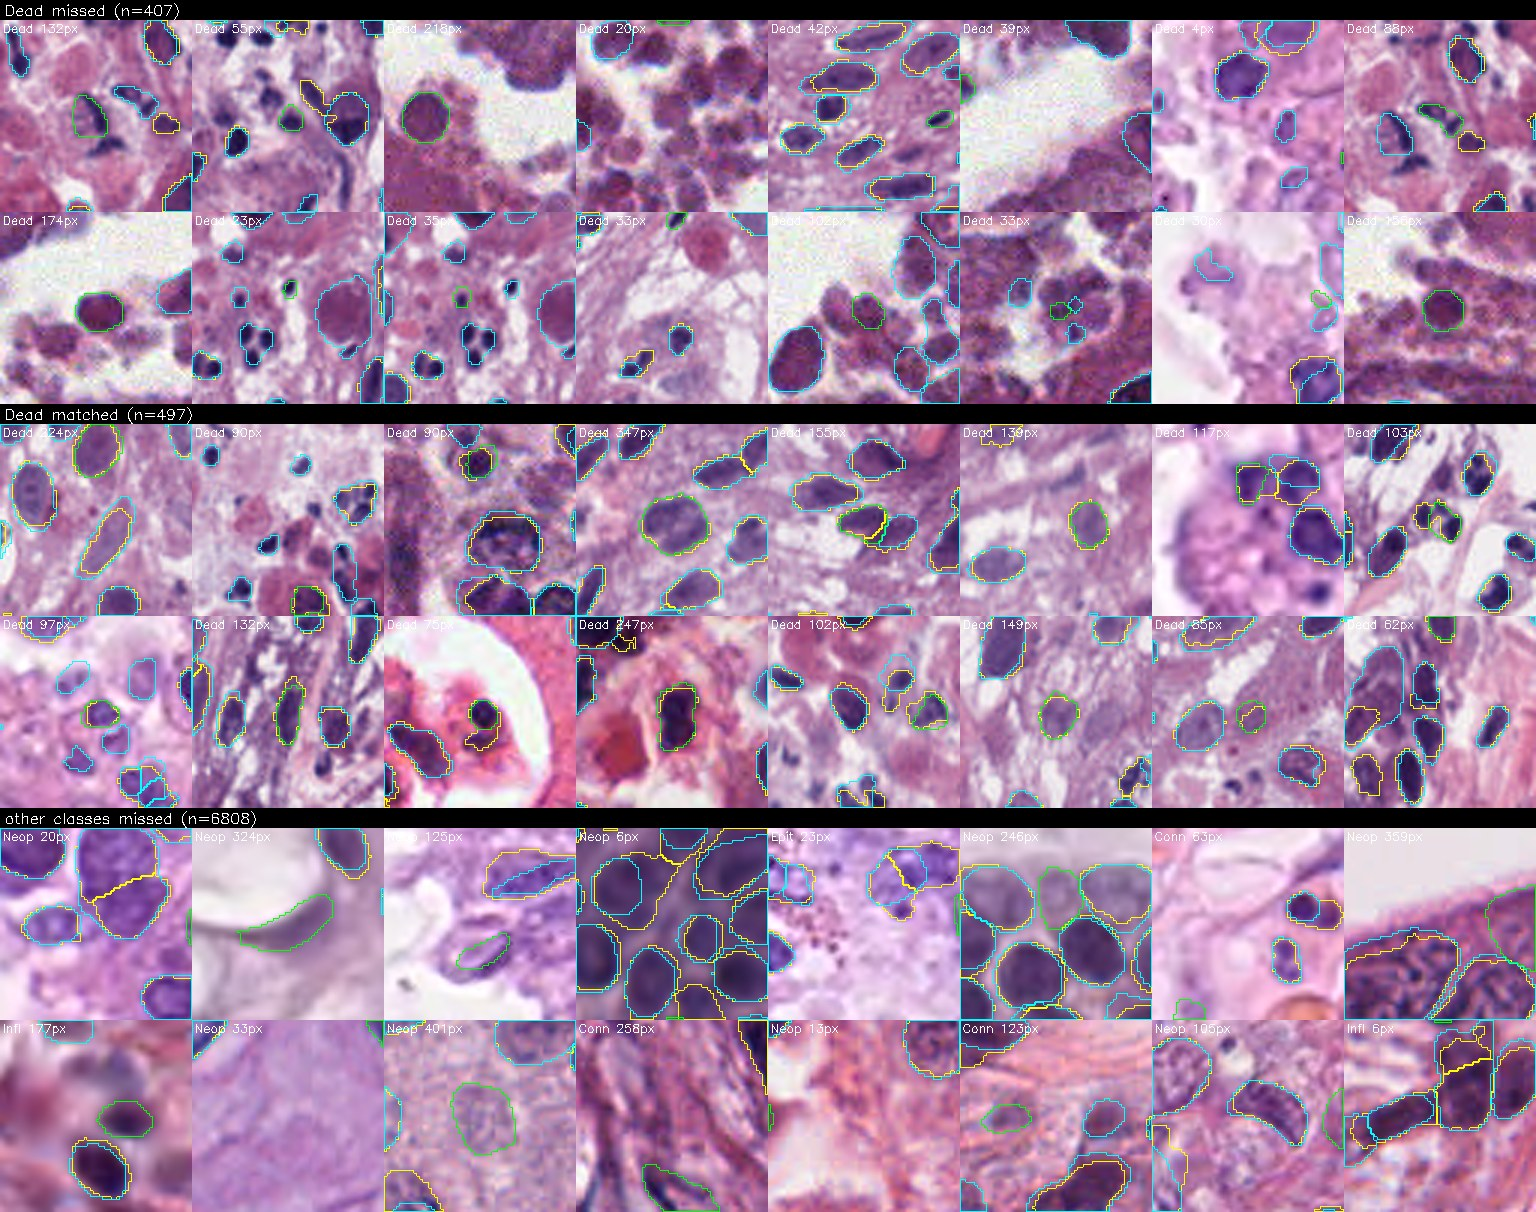
\includegraphics[width=0.86\linewidth]{figs/dead_missed.jpg}
\caption{Dead 真值核（绿色）与预测（黄色），CellViT-UNI 折 3：漏检 Dead 是没有前景响应
的微小暗色碎片与乏染色质凋亡小体。}
\label{fig:dead}
\end{figure}

\section{支柱 B：失败驱动的合成同样无法修复检测}
\label{sec:pillarB}

\subsection{失败布局长什么样}
折外失败挖掘（split-2 模型预测折 1；折 3 测试上模式相同）：漏检 Dead 是\emph{孤立}的
——零接触邻居的 Dead 漏检率 0.39--0.42（占全部 Dead 的约 90\%），漏检 Dead 与其它核接
触的比例 $<$5\%。merge 是同类簇现象（73--82\% 的 merged Dead 与另一 Dead 接触：核碎裂
碎片群）。直觉假设的跨类接触在数据中罕见且不是失败模式。因此原计划的“Dead 紧贴
Neoplastic”干预被替换为：(1) 向空基质插入孤立小核；(2) 密集同类簇。

\subsection{CP1：失败驱动 copy-paste 是有害的}
供体核（50--400\,px，Dead 权重 0.4）以 8\,px 间距粘入无核基质，且在几何/光度增强
\emph{之前}粘贴（粘贴核与宿主 patch 同步增强；v1 的可学习捷径由视觉审查发现并修复，同
时修复的还有边界碎片与未标注核碰撞）。相对 3 种子基线的结果（split 1，测试折 3）：
$\Delta$mPQ $+0.0009$ $[-0.0024,+0.0043]$，但 $\Delta$Dead \textbf{$-0.0310$}
$[-0.0576,-0.0100]$（TTA 一致）。损伤在\emph{分型}而非检测：匹配 Dead 的类型正确率
.690$\rightarrow$.609，混淆双向增加。但验证折在 Dead 上的变化方向恰好\emph{相反}
（$+0.0235$）：Dead PQ 在折间摆动约 0.05，这是噪声规则的第三次独立确认。解释：把真实
外观移植进新上下文，教会模型“干净基质中的孤立小核”是一个偏向 Dead 的线索，从而模糊了类
型边界。

\subsection{上下文内合成（PixCell）：从外观差距到结构性障碍}
PixCell-256 + Cell-ControlNet，以折 1 真实掩码为条件：放置是忠实的（约 95\% 的掩码对象
在正确位置/尺寸渲染，中位 IoU 0.68），但 20$\times$ 生成器在 40$\times$ PanNuke 上有
结构性外观差距（平色块染色质、高频 $-24\%$、大掩码欠渲染且尺寸偏置）。LoRA 适配（两轮，
r16 与 r8 加快照选择）使每个图像空间指标都\emph{更差}，遂放弃该路线；改用对配对真实 patch
的 Reinhard LAB 迁移关闭颜色差距（OD-L1 0.072$\rightarrow$0.009）。锁定配方（基座 +
配对上下文 + Reinhard）下，32 张图的冒烟测试通过视觉审查（颜色与配对真实相差约 3/255），但审
查暴露了一个结构性障碍：ControlNet 条件是\emph{二值}掩码，上下文 embedding 不含类别信
息——生成器无法表达类别特定的外观——729 个保留对象中 0 个被教师判为 Dead
（P(Dead)$\le 0.005$）。强行使用供体类别标签会原样复现 CP1 的失败（标签与外观矛盾）。
SYN1 因此采用\emph{类别无关、教师自洽}的标签——它只能通过检测环节起作用：1146 张合成图以
50\% 混合，其余与基线配方完全一致。结果（测试折 3）：mPQ 0.4900 vs 基线 0.4951（3 种子
区间 0.4910--0.4951 的底部），Dead 0.1521 vs 0.1424（约 $+1$ 点，处于种子噪声边缘；
PQ$^+$/DQ$^+$/SQ$^+$ 全平：这点 Dead 收益来自更好的类型配对而非更好的分割），Inflammatory
$-1.0$--$1.6$ 点。按预注册规则判定：无效。

\begin{figure}[t]
\centering
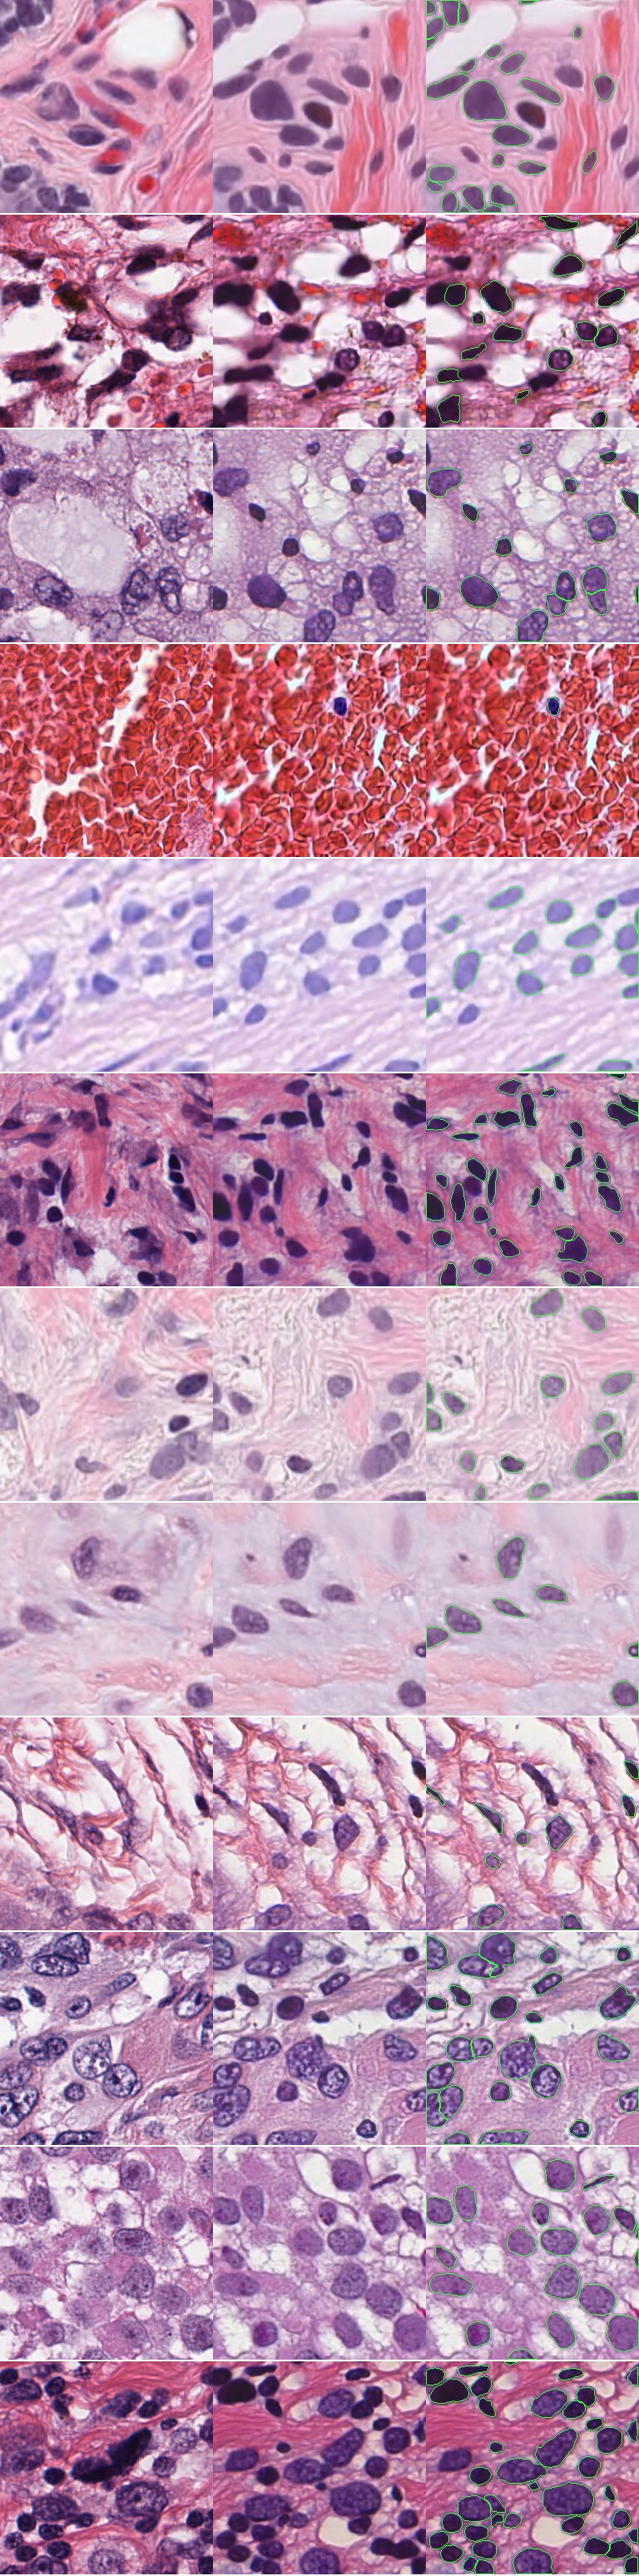
\includegraphics[width=0.30\linewidth]{figs/synth_v2.jpg}
\caption{SYN-v2 合成样例（真实 $|$ 生成 $|$ 标签）：配对上下文 + Reinhard 下外观通过审
查，但二值掩码条件使生成器无法表达类别定向外观（没有生成对象可读作 Dead）。}
\label{fig:synth}
\end{figure}

\subsection{支柱 B 判定}
在不重训生成器条件的前提下，Dead/小核检测缺陷无法被现有的数据侧手段修复：真实外观移植
（CP1）反而损害 Dead 分型，标签自洽的上下文内合成（SYN1）无效。连同支柱 A 的无效结果
（重分类、找回、损失重加权），该缺陷看起来是架构性的。

\section{支柱 C：跨域与反事实评测}
\label{sec:pillarC}

\subsection{真实跨域零样本：$3{\times}3$}
\label{sec:external}

外部数据集（已转换并通过拼接图审查）：\textbf{CoNIC}（19,476 tiles；剔除 112 张源自
PanNuke 的 patch；20$\times\rightarrow$2$\times$ 上采样；类 Inflam/Epith/Conn）、
\textbf{MoNuSAC} test（443 tiles；Inflam/Epith）、\textbf{PUMA} 黑色素瘤（3,278 tiles；
PanNuke 5 类齐全，含 1,991 个凋亡$\rightarrow$Dead 核——我们找到的唯一较大外部 Dead 来
源；GT 由 HoVer-Net 初始化、病理学家校正，绝对召回有上限，但这一上限对所有模型一视同仁）。

\begin{table}[t]
\centering\small
\caption{零样本跨域（3-split 均值，无 TTA）。域内 mPQ：CellViT 0.4995、HoVer-Net
0.4564、HoVer-NeXt-T 0.4579。}
\label{tab:external}
\begin{tabular}{llccc}
\toprule
模型 & 数据集 & mPQ & bPQ & $F_d$ \\
\midrule
CellViT-UNI  & CoNIC   & .3351\,$\pm$.0037 & .5314 & .7816 \\
             & MoNuSAC & .2495\,$\pm$.0218 & .5616 & .7652 \\
             & PUMA    & .4518\,$\pm$.0031 & .7177 & .8831 \\
\midrule
HoVer-Net    & CoNIC   & .2610\,$\pm$.0061 & .5136 & .7669 \\
             & MoNuSAC & .0370\,$\pm$.0003 & .2756 & .3658 \\
             & PUMA    & .3203\,$\pm$.0139 & .7136 & .8714 \\
\midrule
HoVer-NeXt-T & CoNIC   & .2786 & .4811 & .725 \\
             & MoNuSAC & .1123 & .4025 & .628 \\
             & PUMA    & .3813 & .6888 & .848 \\
\bottomrule
\end{tabular}
\end{table}

表~\ref{tab:external}：所有模型都退化，但方式不同。HoVer-Net 在 MoNuSAC 上几乎
\emph{崩溃}（$F_d$ 0.37；各 split 0.26--0.78）：检测失败。PUMA 上没有模型检测崩溃
（$F_d$ 0.85--0.88）——损失在\emph{分型}（HoVer-NeXt-T strict mPQ 0.31 vs mPQ 0.38），
且尽管有 1,991 个凋亡真值核，\textbf{三架构的 Dead PQ 均 $\le$0.006}：Dead 失效模式跟随
模型跨域。TTA 无法挽救迁移（CoNIC $+0.005$，MoNuSAC $-0.001$）。真实跨域降幅（域内 mPQ 减外部均
值）排出的架构次序为 CellViT 0.152 $<$ HoVer-NeXt-T 0.199 $<$ HoVer-Net 0.246，在每个
数据集上一致。

\subsection{PanNuke-CF：标签固定的反事实渲染}
\label{sec:cf}

\begin{figure}[t]
\centering
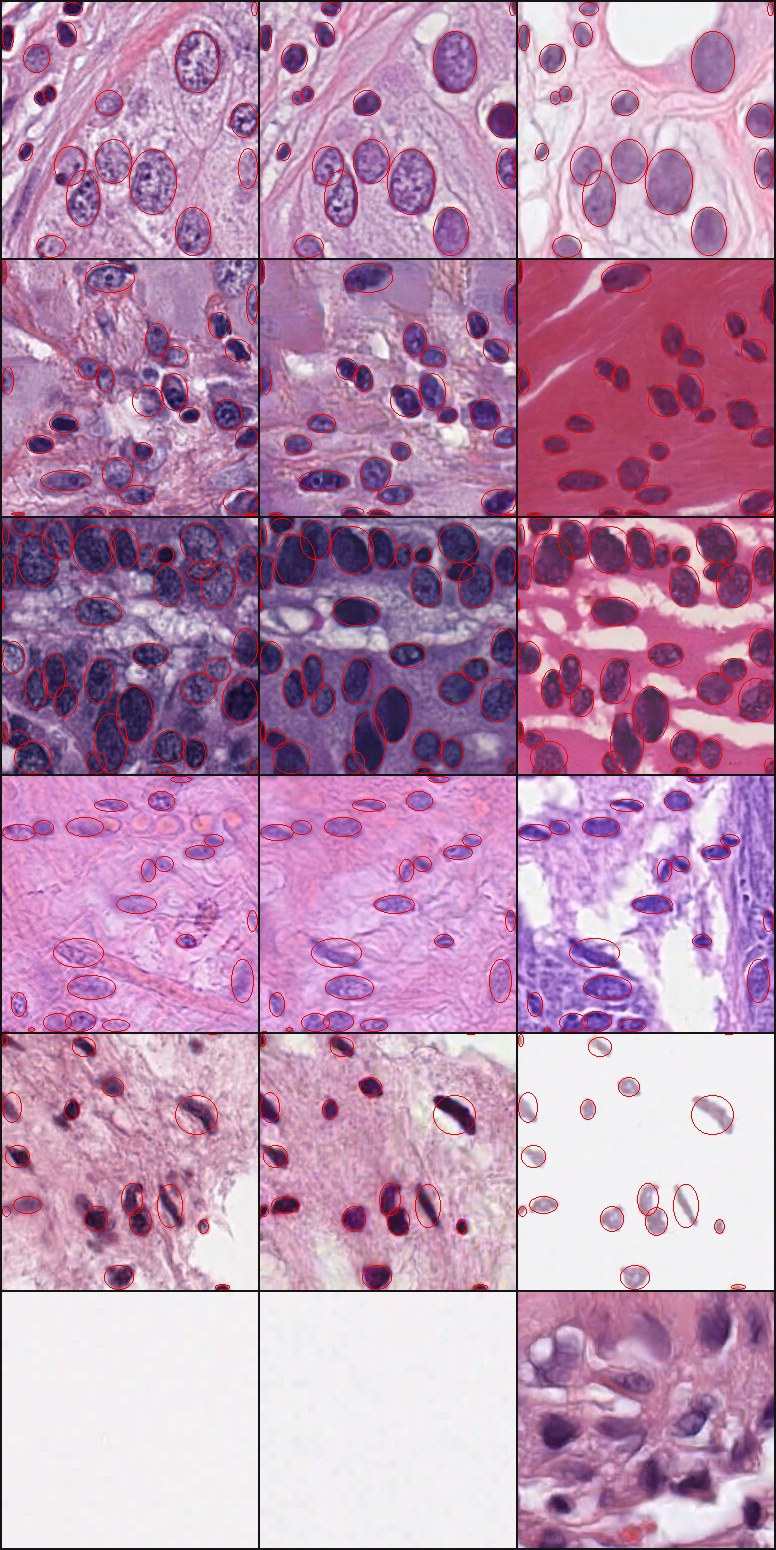
\includegraphics[width=0.42\linewidth]{figs/cf_arms.jpg}
\hfill
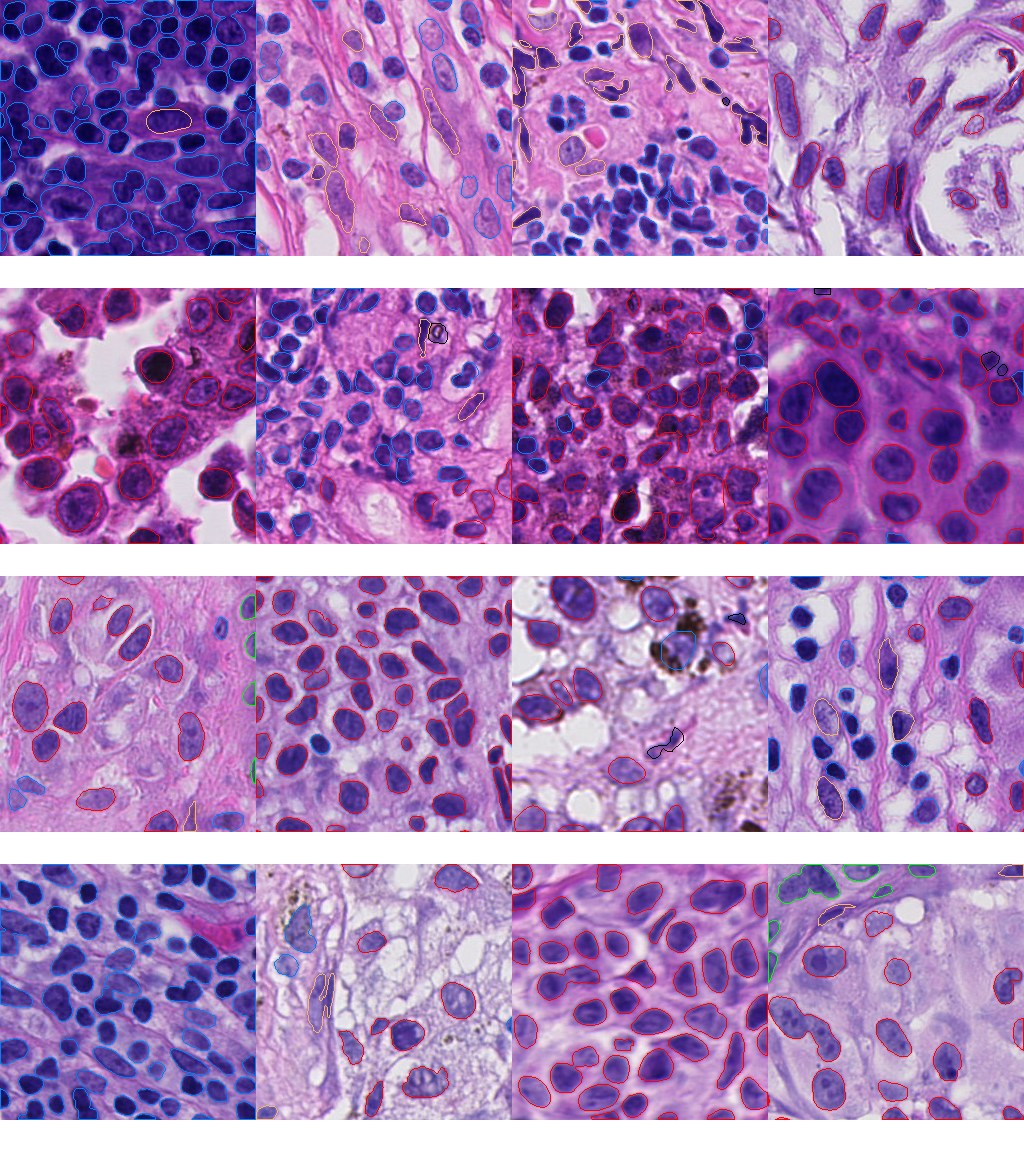
\includegraphics[width=0.42\linewidth]{figs/puma_gt.jpg}
\caption{左：PanNuke-CF 各臂（同一折 3 GT 标签在上下文/染色干预下重渲染）。右：PUMA
真值（类别着色；黑轮廓 = 凋亡 Dead），提供跨域 Dead 标签的外部集。}
\label{fig:cf}
\end{figure}

500 张折 3 patch，\emph{GT 标签固定}，由（冻结）生成器在因子化外观干预下重渲染——上下文
\{配对， 换组织\} $\times$ Reinhard 目标 \{自身， donor\}——得到
\texttt{control}/\texttt{stain}/\texttt{ctx}/\texttt{tissue} 四臂，外加未经改动的
\texttt{real} 原图与 3 个生成器种子的 control 重复（噪声底）。生成器噪声比下述效应小一
个数量级（control 重复 mPQ std 0.002--0.006）。两个标定事实：生成的 \texttt{control} 图
像比真实\emph{更容易分割}（bPQ 0.78 vs 0.67），但携带\emph{类型不一致}的外观（strict
mPQ 0.36 vs 0.45）——因此 CF 比较永远是臂对 control，绝不直接对 real；空白 patch 必须剔
除（上下文 embedding 是内容通道）。

\begin{table}[t]
\centering\small
\caption{PanNuke-CF，架构在 2 个 split 上的均值（mPQ；括号为相对 control 均值的配对
$\Delta$，图像 bootstrap 95\% CI 除 HoVer-NeXt-T stain 外均不含 0）。}
\label{tab:cf}
\begin{tabular}{lccccc}
\toprule
架构 & real & control & stain & ctx & tissue \\
\midrule
CellViT-UNI  & .495 & .449 & .426 [$-$.023] & .259 [$-$.190] & .258 [$-$.191] \\
HoVer-Net    & .449 & .439 & .373 [$-$.066] & .300 [$-$.140] & .293 [$-$.146] \\
HoVer-NeXt-T & .456 & .425 & .417 [$-$.008] & .262 [$-$.163] & .261 [$-$.164] \\
\bottomrule
\end{tabular}
\end{table}

上下文交换是强压力源（Epithelial PQ 崩塌 0.24--0.43，而 $F_d$ 只降 0.08--0.10：它摧毁
的是\emph{类型}信息），染色是弱压力源。需要检验的问题是：这些反事实降幅能否在评估器之间预测
\emph{真实}的跨域降幅。

\subsection{有效性：反事实压力反转真实排序}
\label{sec:validity}

在 6 个评估点（3 架构 $\times$ 2 splits）上，CF 降幅对比真实跨域降幅：Spearman
$\rho=-0.89$（\texttt{ctx}，精确置换 $p=0.033$），\texttt{tissue} $-0.89$，
\texttt{stain} $+0.43$ 不显著。在架构均值上（这是更诚实的检验；同一架构的两个 split 近乎重复）
ctx 与 tissue 都给出 $\rho=-1.00$：完全倒置——域内最受上下文交换伤害的模型
（CellViT）是真实迁移中最鲁棒的，反之亦然。

\begin{table}[t]
\centering\small
\caption{轴分解（架构均值）：每个降幅拆为检测（$F_d$）与分型（bPQ$-$mPQ 间隙增量）。
架构间的真实迁移差异位于检测轴，而 CF 压力在检测轴上架构齐平。}
\label{tab:axes}
\begin{tabular}{lcc|cc|cc}
\toprule
& \multicolumn{3}{c|}{真实（域内 $-$ 外部）} & \multicolumn{3}{c}{CF ctx（control $-$ ctx）} \\
架构 & mPQ & $F_d$ & 分型 & mPQ & $F_d$ & 分型 \\
\midrule
CellViT-UNI  & .154 & \textbf{.007} & +.088 & .190 & .102 & +.082 \\
HoVer-Net    & .246 & \textbf{.163} & +.069 & .140 & .084 & +.034 \\
HoVer-NeXt-T & .199 & \textbf{.045} & +.085 & .163 & .090 & +.064 \\
\midrule
\multicolumn{7}{l}{\footnotesize 轴匹配 rank agreement（全部 6 点 / 架构均值）：}\\
\multicolumn{7}{l}{\footnotesize\quad mPQ：$-0.89$（$p{=}.033$）/ $-1.00$；\quad
检测 $F_d$：$-0.83$（$p{=}.058$）/ $-1.00$；\quad 分型：$+0.71$ / $\mathbf{+1.00}$。}\\
\bottomrule
\end{tabular}
\end{table}

表~\ref{tab:axes} 给出机理。架构间的真实迁移差异集中在\emph{检测}轴（CellViT 的 $F_d$
损失 0.007；HoVer-Net 0.163——其 MoNuSAC 崩溃），分型间隙增量则彼此接近
（0.07--0.09）。但标签固定的渲染\emph{无法}对检测施压：生成器在固定位置重渲染形态完好
的核，CF 的 $F_d$ 降幅因此在架构间齐平（0.08--0.10），不携带排序信息。在 CF \emph{能}
施压的地方——上下文/染色错配下的分型——其排序与真实分型迁移一致（架构均值
$\rho=+1.00$；全部 6 点 $+0.71$/$+0.83$）。必须指出的局限：$n=3$ 个架构（架构均值
$|\rho|=1$ 对应的精确 $p=1/3$；更有力的证据是 3 架构 $\times$ 2 splits 的完全符号倒置加上
轴分解机理），且架构间真实分型差异（区间 0.069--0.088）远小于检测差异（0.007--0.163）。

\paragraph{判定。}PanNuke-CF 是有效的\emph{分型压力测试}——它与真实迁移一致地排序各架
构的分型鲁棒性——但它\emph{不是}迁移代理：当作代理使用会反转排序，因为其盲区（检测）恰
是真实迁移差异所在。仅干预外观的反事实天然带有这一构造性限制；探测检测鲁棒性需要对
\emph{布局}（密度、杂乱、伪影）的干预，而非外观。

\section{讨论}
\label{sec:discussion}

\paragraph{为什么三个支柱都以负结果收场。}三个支柱共享一个隐含假设——Dead 性能受限于信息
（语言先验）或数据（合成样本），而非检测架构。诊断给出了相反的证据：漏检 Dead 核在 83\%
的像素上没有前景响应，类型分支却已经“看见”它们；语言侧融合、后处理找回、损失重加权
（3 种子）、真实外观移植、标签自洽的上下文内合成都未能撼动检测。该缺陷与 40$\times$ 下
NP 头的分辨率/架构相符——这是一个我们尚未在架构上检验的假设（如更高分辨率的前景监
督），也是主要的开放方向。

\paragraph{评测方法论。}三条教训，均有证据支撑：(1) PanNuke 的种子噪声依赖类别（mPQ 0.002 vs
Dead 0.007），且验证折的 Dead 信号可能与测试相反（CP1：$+0.024$ vs $-0.031$）——单种子、
单折的 Dead 结论不可信；(2) 已发布的评测配方可能内嵌相当于约 0.02 mPQ 的测试侧调参收益
（我们的 HoVer-NeXt-T 解码研究），大于排行榜的典型名次差距；(3) 生成的评测数据系统性地
\emph{更易分割}但\emph{类型一致性更差}，因此反事实基准必须臂对 control 评分，并同时报
告 strict mPQ 与 mPQ。

\paragraph{Dead 作为跨域现象。}三架构在 PUMA 上 Dead PQ $\le$0.006——尽管 Dead 是 CONCH
最可文本识别的类，也是我们域内模型检出后能以 0.69 正确分类的类——说明域内的 Dead 线索
（40$\times$ 下的深色固缩染色质）不迁移到黑色素瘤 H\&E 中的凋亡小体。任何针对 Dead 的
改进都必须经过跨域验证，而不只在 PanNuke 折上。

\section{状态与后续工作}
\label{sec:status}

所有预注册实验已完成：基线复现（课程要求 (a)、(b) 完成），错误分解与类$\times$组织分析
完成（(c)），支柱 A/B 以负结果收官，支柱 C 以一个机理性的评测结果收官。最终报告还需要：三架构的
组织$\times$类热力图与错误分解图、精简的主表集合、可选的额外外部集（MoNuSeg、
NuInsSeg；仅 bPQ/AJI）、以及文字润色。可选的开放方向（未预注册）：从架构侧着手解决 Dead 检
测缺陷，以及布局干预反事实——探测仅外观 CF 无法触及的检测轴。

\begin{thebibliography}{99}\small
\bibitem{gamper2019pannuke} J.~Gamper et al., ``PanNuke Dataset Name, Instance Segmentation and
Classification in Hematoxylin \& Eosin Stained Histology Images,'' \emph{Medical Image Analysis},
2020.
\bibitem{graham2019hovernet} S.~Graham et al., ``HoVer-Net: Simultaneous Segmentation and
Classification of Nuclei in Multi-Tissue Histology Images,'' \emph{Medical Image Analysis}, 2019.
\bibitem{horta2024cellvit} J.~S.~Horta~Malo et al., ``CellViT: Vision Transformers for Precise
Cell Instance Segmentation,'' \emph{Medical Image Analysis}, 2024. arXiv:2306.15350.
\bibitem{horta2025cellvitpp} J.~S.~Horta~Malo et al., ``CellViT++,'' arXiv:2501.05269, 2025.
\bibitem{hovenext} S.~D.~Bhattacharjee et al., ``HoVer-NeXt: Exploring Reliable and Efficient
Lifted ViT Baselines for Nuclei Segmentation,'' \emph{MIDL}, 2024.
\bibitem{cppnet} Y.~Zhou et al., ``CPP-Net: A Unified Framework for Nuclei Instance Segmentation
and Classification,'' arXiv:2102.06867, 2021.
\bibitem{promptnucseg} S.~Graham et al., ``PromptNucSeg: A Text-Driven Nuclei Instance
Segmentation Method,'' \emph{ECCV}, 2024. arXiv:2311.15939.
\bibitem{lu2024conch} R.~Lu et al., ``A Visual-Language Foundation Model for Computational
Pathology (CONCH),'' \emph{Nature Medicine}, 2024. arXiv:2307.12914.
\bibitem{mindthegap} ``Mind the Gap: Meta-Analysis of Foundation Models for Pathology Image
Analysis,'' arXiv:2502.02471, 2025.
\bibitem{le2025pixcell} M.~Le et al., ``PixCell: A Generative Model for Digital Pathology
Slides,'' arXiv:2506.05127, 2025.
\bibitem{nucleimix} ``NucleiMix: Diffusion-Based Rare-Nuclei Synthesis,'' arXiv:2410.16671, 2024.
\bibitem{cfstress} ``Counterfactual Stress Testing of Medical Imaging Models,'' arXiv:2605.10894, 2026.
\end{thebibliography}

\end{document}
